\documentclass[aps,reprint,amsmath,amssymb,showpacs,showkeys]{revtex4-1}% APS journal style
\usepackage{graphicx}% Include figure files
\usepackage{dcolumn}% Align table columns on decimal point
\usepackage{bm}% bold math
\usepackage{hyperref}% add hypertext capabilities
\usepackage{natbib}  % Package for Bibtex
%\usepackage{amsmath}  % Package for typesetting formulae
%\usepackage{amssymb}  % Package for some math symbols and fonts
\usepackage[justification=justified]{caption}
%\usepackage[caption=false]{subfig}
\usepackage{subcaption} % subfigure
\usepackage{amsopn}
\usepackage{float}
\usepackage{tikz}
\usetikzlibrary{shapes.geometric, arrows}
\tikzstyle{sqr2} = [rectangle, minimum width=3.5cm, minimum height=0.9cm, text centered, draw=black, fill=yellow!30]

\usepackage{ulem} % \sout function
\usepackage{booktabs} % Top and bottom rules for tables

%\usepackage{breqn}

\newcommand{\bt}[1]{\ensuremath{\mathbf{#1}}}  % bold math
%\newcommand{\bm}[1]{\mbox{\boldmath $#1$}}
\newcommand{\cb}{ \color{blue}}
\newcommand{\cred}{\color{red}}
\newcommand{\jv}[1]{\textcolor{cyan}{JV: #1}}
\newcommand{\Msun}{$\text{M}_{\odot}$}

\begin{document}
\graphicspath{{figures/}}	

% Define author, title, and date
\title[Spectral density estimation using P-spline priors]{Spectral density estimation using P-spline priors}

\author{Patricio Maturana-Russel$^{1}$ and Renate Meyer$^1$}
\affiliation{$^1$ Department of
  Statistics, University of Auckland, Auckland 1142, New Zealand}


\begin{abstract}
This article proposes a P-spline prior to estimating the spectral density of a stationary time series.  Our proposal is a particular case of the B-spline prior algorithm.  We assess our proposal via a simulation study and two real data sets.
\end{abstract}

\pacs{04.30.-w, 02.50.-r, 05.45.Tp, 97.60.Bw}

\keywords{P-spline prior, B-spline prior, spectral density estimation, Whittle likelihood}


\maketitle

\section{Introduction}
The power spectral density (PSD), or simply spectral density, describes the distribution of the power or variance for each individual frequency composing a time series.  It embodies useful information for the study of stationary time series.  An absolutely summable autocovariance function, that is $\sum_{h=-\infty}^{\infty} |\gamma(h)| <\infty$, guaranties the existence of the spectral density function of a zero-mean weakly stationary time series, being continuous, bounded and given by
\begin{align*}
f(\lambda) = \dfrac{1}{2\pi} \sum_{h = -\infty}^{\infty}\gamma(h)\exp\left(-i h \lambda \right), 
\end{align*}
where $-\pi < \lambda \leq \pi$ is the angular frequency.

Methods to estimate this function go from parametric to nonparametric approaches.  The former are basically based on autoregressive moving average (ARMA) models.  As any parametric model, the results tend to be biased if the model approximation to the underlying time series is poor.  

Most of the nonparametric methods work by smoothing the periodogram
\begin{align*}
I_n(\lambda) = \dfrac{1}{2 \pi n} \left| \sum_{t=1}^{n} Y_t \exp \left( -i t \lambda\right)\right|^2,
\end{align*}
where $-\pi < \lambda \leq \pi$ is the angular frequency and $Y_t$ is a stationary time series of length $n$, because this fluctuates around the true spectral density function.  This function has interesting features, for instance, it is asymptotically unbiased and follows an exponential distribution with mean $f(\lambda)$.  However, it is not consistent \citep{Brockwell:1986}.

Bayesian nonparametric approaches for spectral density estimation allow the data to determine the complexity of the model.  These approaches avoid the comparison of models which vary in complexity and adapt a single model according to the data. \cite{Gangopadhyay:1999} fitted a fixed low order piecewise polynomials to the log-spectral density function, allowing free known number and location of knots.  For this, a reversible jump Markov chain Monte Carlo (RJMCMC) \citep[RJMCMC;][]{Green:1995} algorithm was used.

\cite{Choudhuri:2004} allocated a Bernstein polynomial as prior on the spectral density function.  This prior is a mixture of beta densities weighted by a Dirichlet process.  The number of components, which is a smoothing parameter, has a discrete prior.  \cite{Edwards2018} extended the method replacing the beta densities for B-spline functions.  These functions have the advantage of having local support, unlike the beta densities, which allow more flexibility and have the potential of modelling spectral densities with sharp and abrupt changes.  Thus, the B-spline prior outperforms the Bernstein polynomial in estimating complex PSDs \citep{Edwards2018}.  However, this flexibility comes with a much higher computational cost.

The Bernstein polynomial and the B-spline methods make use of Whittle's approximation to the Gaussian likelihood, known simply as Whittle likelihood \citep{Whittle:1957}.  One of the advantages of this approximation is that involves directly the spectral density, unlike the true likelihood function.

Taking advantage of the limiting independent exponential distribution of the periodogram, the Whittle likelihood for a mean centred weakly stationary time series $\bm{Y}$ of length $n$ is defined as
\begin{align}
 L(\bm{Y} | f) &= \prod_{l=1}^{\nu}\dfrac{1}{f(\lambda_{l})} e^{-I_n(\lambda_l)/f(\lambda_l)}  \nonumber \\
 &\propto \exp \left( - \sum_{l=1}^{\nu} \log f(\lambda_l) + \dfrac{I_{n}(\lambda_l)}{f(\lambda_l)} \right), \label{eq:whittle_like}
\end{align}
where $\lambda_l = 2\pi l / n$ are the Fourier frequencies, $f(\cdot)$ spectral density of $\bm{Y}$, and $\nu = \left\lfloor (n-1)/2 \right\rfloor$ is the greatest integer value less than or equal to $(n-1)/2$.

Motivated by the flexibility of the B-spline prior and its associated high computational cost, in this work, we implement and test a particular case of the B-spline prior.  For this, we fix the number of B-spline densities and place a P-spline prior on the spectral density instead.  This approach allows to penalize automatically the inclusion of B-spline densities and save significantly computational time without sacrificing accuracy.  Actually, as will show, it outperforms the B-spline prior in our tests.  In addition, we propose a knot location scheme based on the periodogram, which aims to deal with PSD shapes that possess  abrupt peaks, without increasing computational time.  We show in an example how this scheme improves significantly the estimates.

We start defining the B-spline densities and the B-spline prior. Then, we define the P-spline prior and discuss its implementation.  Finally, we test our approach and compare it to the B-spline prior in a simulation study, and two real problems.

\section{B-spline prior}

A mixture of beta densities with only integer parameters can approximate uniformly any continuous density on $[0,1]$.  Let $G$ be a cumulative distribution function (cdf), with continuous density $g$, then 
\begin{align*}
\widehat{G}(\omega) &= \sum_{k=1}^{K} G \left( \dfrac{k-1}{K} , \dfrac{k}{K} \right] \beta(\omega; k, K-k+1)\\
&= \sum_{k=1}^{K} w_k \beta(\omega; k, K-k+1)
\end{align*}	  
converges uniformly to $G(\omega)$, where $G(u,v] = G(v) - G(u)$ and $\beta(\omega; a,b)$ is the beta density with parameters $a$ and $b$.
The Bernstein polynomial prior, which is used to describe a nonparametric prior for probability densities in the unit interval, is based on this approximation \citep{Petrone:1999a,Petrone:199b}.  \cite{Choudhuri:2004} proposed it as a prior on the spectral density function.

As shown by \cite{Perron:2001}, the mixture of beta distributions is unable to provide a full coverage of the space of cdfs on $[0,1]$.  They defined a loss function and showed that this cannot be arbitrarily small under this approach.  Alternatively, they showed that if the beta distributions are replaced by B-spline distributions of fixed order (shown for order~2) with variable knots, the loss function can be arbitrarily small by increasing the number of knots.  The adequacy of the approximation is a function of the number of knots.  This work motivated \cite{Edwards2018} to propose the B-spline prior on the spectral density function.

\subsection*{B-splines}

A spline of degree $r+1$ is a function defined piecewise by polynomials of degree $\leq r$, which meet at points called \textit{knots} where the function is continuous.  Any of these spline functions can be described by basis functions, known as \textit{B-splines}, in other words, all spline functions can be represented as a unique combination of B-splines with the same order and over the same partition.  Without loss of generality, the global domain of interest is assumed to be the unit interval $[0,1]$.

The B-spline basic functions of any order can be recursively defined as
\begin{align*}
	B_{k,0}(\omega, \bm{\xi})=&	
	\left\{
	\begin{array}{ll}
		1, & \omega \in [\xi_{k-1}, \xi_{k}] \\
		0, & \mbox{otherwise} 
	\end{array}
	\right.\\
	B_{k,r}(\omega, \bm{\xi}) = & \:v_{k,r}B_{k,r-1}(\omega; \bm{\xi}) + \\
	   & \: (1-v_{k+1,r})B_{k+1,r-1}(\omega; \bm{\xi}),	
\end{align*}
where	   
\begin{align*}	   
	v_{k,r}&=	
	\left\{
	\begin{array}{ll}
		\dfrac{\omega - \xi_{k-1}}{\xi_{k+r-1} - \xi_{k-1}}, & \xi_{k-1} \neq \xi_{k+r-1}\\
		0, & \mbox{otherwise} 
	\end{array}
	\right.
\end{align*}
and 
\begin{align*}
	\bm{\xi} = \{0 = \xi_0 = \xi_1 = \cdots = \xi_r \leq \xi_{r+1} \leq \cdots \leq \xi_{K}\\ = \xi_{K+1} = \cdots = \xi_{K+r} = 1 \}
\end{align*}
is the knot vector.  This vector is a non-decreasing sequence that contains $K+r+1$ knots, which can be divided in $2(r+1)$ external and $K-r-1$ internal knots.  The latter must be $\geq r$.

The \textit{B-spline densities}, normalized B-spline functions, are defined by
\begin{align*}
	b_{k,r}(\omega; \bm{\xi}) = \left(r+1\right) \dfrac{B_{k,r}(\omega;\bm{\xi})}{\xi_{k+r} - \xi_{k-1}}.
\end{align*}

% include reference for the normalizing constant

\subsection*{Prior description}
The B-spline prior is a mixture of B-spline densities defined as
\begin{align}
s_r(\omega; K,\bm{w}_K, \bm{\xi}) = \sum_{k=1}^{K} w_{k,K} b_{k,r}(\omega;\bm{\xi}),
\label{eq:bs_prior}	
\end{align}
where $K$ is the number of B-spline densities  $b_{k,r}(\cdot)$ of fixed degree $r$, $\bm{w}_K=(w_{1,K},\cdots, w_{K,K})$ the weight vector, and $\bm{\xi}$ is the knot sequence.

If the number of B-spline densities $K$ is considered as another parameter, the $\bm{w}_K$ dimension changes according to it.  A natural way to deal with it is the RJMCMC~\citep{Green:1995} algorithm, which was implemented by \cite{Gangopadhyay:1999} in the similar context of low-order polynomials.  However, the method often has implementation difficulties which vary from problem to problem, such as trans-dimensional jumps.

Assuming that the weights are induced by a cdf $G$ on $[0,1]$, \cite{Choudhuri:2004} proposed a Dirichlet process as a prior for the latter.  This approach avoids the potential difficulties caused by the parameter dimension changes associated to RJMCMC.  \cite{Edwards2018} followed this approach, but in addition they assumed that the $K-r$ internal knot differences are induced by a cdf $H$ on $[0,1]$, for which was allocated another Dirichlet prior, that is
\begin{align*}
\Delta_{j} = \xi_{j+r} - \xi_{j+r-1} = H\left(\dfrac{j-1}{K-r}, \dfrac{j}{K-r} \right],
\end{align*}
for $j=1,\dots,K-r$.

Therefore, the B-spline prior on the spectral density function parametrized in terms of $K$, $G$, and $H$ is given by
\begin{align*}
s_r(\omega;K,G,H) = \sum_{k=1}^{K} G \left( \dfrac{k-1}{K} , \dfrac{k}{K} \right] b_{k,r}(\omega;H).
\end{align*}

The B-spline prior is a mixture of B-spline densities with local support, unlike the Bernstein polynomial prior which uses beta densities with full support on the unit interval.  This feature allows the B-spline method more flexibility for spectral density estimation \citep{Edwards2018}.

When there are no internal knots, the B-spline basis turn into the Bernstein polynomial basis.  Therefore, the B-spline prior can be considered as a generalization of the Bernstein polynomial prior.  

%\subsection*{Prior for the spectral density}

The prior discussed above has been defined for the unit interval $[0,1]$.  However, the spectral density function $f(\cdot)$ is defined on the interval $[0,\pi]$, therefore its prior is reparametrized and defined as
\begin{align*}
f(\pi \omega) = \tau \times s_r(\omega;K,G,H), \quad \omega \in [0,1],
\end{align*}
where $\tau = \int_{0}^{1}f(\tau \omega)\text{d}\omega$ is the normalizing constant.

To sum up, the prior has the following components:
\begin{itemize}
	\item $G \sim \text{DP}(M_G, G_0)$, where $M_G>0$ is the concentration parameter and $G_0$ is the base distribution.  It produces the weights for the $K$ B-spline densities.  
	\item $H \sim \text{DP}(M_H, H_0)$, where $M_H>0$ is the concentration parameter and $H_0$ is the base distribution.  It produces the knot locations determining the shape and location of the B-spline densities.
	\item $p(K) \propto \text{exp}(-\theta_K K^2)$ for $K=1,\dots,K_{\text{max}}$.  $K$ is the number of B-spline densities used in Eq. \eqref{eq:bs_prior}.  It plays the role of smoothing parameter, that is smaller values implies smoother spectral density estimates.  $K_{\text{max}}$ must be limited  for computational reasons.  In practice, pilot runs are used to determine it.
	\item $\tau \sim \text{Inverse-Gamma}(\alpha_{\tau},\beta_{\tau})$ is the normalizing constant.  $\alpha_{\tau}$ and $\beta_{\tau}$ are the shape and scale parameters, respectively.
\end{itemize}

\subsection*{Implementation discussion}

The B-spline prior proposed by \cite{Edwards2018} involves 2 Dirichlet processes placed on $G$ and $H$, the weights of the B-spline densities and the knot locations, respectively.  The sampling from them is carried out by the stick-breaking construction \citep{Sethuraman:1994}.  This method consists basically in a representation of the Dirichlet process as a sequential division of the unit interval infinite times according to a beta distribution.  For computational reasons, the number of components of this representation of $G$ and $H$ is limited to a large but finite positive integer, that is $L_G$ and $L_H$, respectively.  These parameters control the quality of the approximations.  Larger values improve the approximation, but increase the number of calculations and consequently the computation time.

The stick-breaking approximation requires the re-parametrization of $G$ to $(Z_0,Z_1,\dots, Z_{L_G},V_1,\dots,V_{L_G})$, which are all independent, such that
\begin{align*}
G&=\sum_{l=1}^{L_G} p_l \delta_{Z_l} + \left(1- \sum_{l=1}^{L_G} p_l\right)\delta_{ Z_{0}},
%p1 &= V_1, \\
%p_l&=\left( \prod_{j=1}^{l-1} (1 - V_j) \right) V_l, \quad l \geq 2\\
%p_0&=1-\sum_{l=1}^{L_G}p_l,\\
%V_l &\sim \text{Beta}(1,M_G), \quad l=1,\dots,L_G,\\
%Z_l &\sim G_0, \quad l = 0,1\dots,L_G.
\end{align*}
where $p_1 = V_1$, 
\begin{align*}
p_l &= V_l \prod_{j=1}^{l-1} (1 - V_j), \:\: \text{for } l \geq 2, \\
p_0 &= 1-\sum_{l=1}^{L_G}p_l,
\end{align*}
$\delta_{Z_{0}}$ is a degenerate probability density, that is $\delta_{Z_0}=1$ at $Z_0$ and 0 otherwise, $V_l \sim \text{Beta}(1,M_G)$, for $l=1,\dots,L_G,$ and $Z_l \sim G_0$, for $l = 0,1\dots,L_G$.  Conditional on $K$, the weights of the B-spline densities are defined as
\begin{align*}
	w_{k,K} = \sum_{l=0}^{L_G}p_l I\left\{ \dfrac{k-1}{K} < Z_l < \dfrac{k}{K}\right\}.
\end{align*}

Analogously, $H$ is re-parametrized as $(X_0,\dots,X_{L_H}, U_1,\dots,U_{L_H})$ by the stick-breaking method truncated at $L_H$.  Thus, the knot differences and consequently the knot locations are defined as
\begin{align*}
\Delta_{j} &= \xi_{j+r} - \xi_{j+r-1} \\
&= \sum_{l=0}^{L_H}q_l I\left\{ \dfrac{j-1}{K-r} < X_l < \dfrac{j}{K-r} \right\},		
\end{align*}
where $q_l$ is defined similarly to $p_l$ that was described above.

As a result, the joint prior for the parameter vector $\bm{\theta} = (\textbf{v},\textbf{z},\textbf{u},\textbf{x},K,\tau)$ is given by
\begin{align}
p(\bm{\theta}) \propto & \left( \prod_{l=1}^{L_G} M_G(1-v_l)^{M_G -1} \right) \left( \prod_{l=0}^{L_G}g_0(z_l) \right) \nonumber \\
&\times \left( \prod_{l=1}^{L_H} M_H(1-u_l)^{M_H -1} \right) \left( \prod_{l=0}^{L_H}h_0(x_l) \right) \nonumber \\
&\times p(K) p(\tau) \label{eq:prior}
\end{align}
An unnormalized joint pseudo-posterior is obtained by multiplying this prior density and the Whittle likelihood defined in Eq. \eqref{eq:whittle_like}.

The sampling is performed via the Gibbs sampling technique.  More details about the MCMC implementation of the B-spline prior method can be found in \cite{Edwards2018}.\\

As shown by \cite{Edwards2018}, the B-spline prior outperforms the Bernstein polynomial prior in estimating spectral densities with sharp and abrupt changes. In the case of simple ones, there is no a significant difference.  However, in practice, this function is unknown, which makes necessary the use of general methods, such as the B-spline prior algorithm.  

The Bernstein polynomial prior requires the calculation of the beta densities only once and they can be re-utilized across MCMC steps.  On the other hand, the B-spline prior method requires the calculation of the B-spline densities at each iteration, since these vary according to the knot locations and the number of B-spline densities.  Moreover, the Dirichlet processes approximated via the stick-breaking method require $2\!\times\!(L_G + L_H)$ calculations (see Eq. \eqref{eq:prior}) at each iteration.  All of this makes the B-spline prior algorithm much more complex in comparison to the Bernstein polynomial prior. 

The complexity of the B-spline prior algorithm is mainly because it allows variable number of B-spline densities $K$.  This has prompted us to the implementation and assessment of the P-spline prior algorithm, which uses a fixed number of B-spline densities and knot locations, avoiding the Dirichlet processes and the recalculation of the B-spline densities.  One of its advantages is that this method keeps the local support of the B-spline densities, unlike the Bernstein polynomials, which can potentially allow to estimate spectral densities with sharp and abrupt changes.

%%%%%%%%%%%%%%%%%
%%% P-splines %%%
%%%%%%%%%%%%%%%%%

\section{P-spline prior}

Fixing the number of B-spline densities $K$ in Eq. \eqref{eq:bs_prior}, the prior for the unit interval $[0,1]$ is defined as
\begin{align*}
	s_r(\omega;\bm{w}, \bm{\xi}) = \sum_{k=1}^{K} w_{k} b_{k,r}(\omega;\bm{\xi}),	
\end{align*}
where $\bm{w} = (w_1,\dots,w_K)$, and $\bm{\xi}$ contains equidistant internal knots on $[0,1]$.  Therefore, the P-spline prior on the spectral density function is given by
\begin{align*}
f(\pi \omega) = \tau \times s_r(\omega;\bm{w}, \bm{\xi}), \quad \omega \in [0,1],
\end{align*}
where $\tau = \int_{0}^{1}f(\tau \omega)\text{d}\omega$ is the normalizing constant.

The roughness penalty in a frequentist context is carried out by penalizing the likelihood function.  In a Bayesian context, this is translated into the prior distribution \citep{Lang:2004} for the $d^{\text{th}}$ order difference of successive weights, known also as B-spline parameters.  

In our approach, we place an indirect prior on the weights
\begin{align*}
\bm{v}&\sim\text{N}_{K-1}(\bm{0}, (\phi \bm{P})^{-1})\\
\phi|\delta &\sim \text{Gamma}(\alpha_{\phi}, \delta \beta_{\phi})\\
\delta &\sim \text{Gamma}(\alpha_{\delta}, \beta_{\delta})
\end{align*}
where $\bm{v} = (v_1,\dots,v_{K-1})^\top$ is a $K-1$ dimensional parameter vector, $\phi$ is the smoothing or penalty parameter, $\textbf{P} = \textbf{D}^\top \textbf{D} +\epsilon \textbf{I}_{K-1}$ is the penalty matrix (full matrix rank matrix for a small quantity $\epsilon$, for instance, $10^{-6}$) with $\textbf{D}$ the $d^{\text{th}}$ order difference matrix, $\alpha_{\phi}$ and $\alpha_{\delta}$ are shape parameters, $\delta \beta_{\phi}$ and $\beta_{\delta}$ are rate parameters, and $\text{Gamma}(a,b)$ denotes a gamma distribution with mean $a/b$ and variance $a/b^2$.

The $1^{\text{st}}$ order difference matrix \textbf{D} is defined as
\begin{align*}
\begin{bmatrix}
-1 & 1   & 0  & 0 & \cdots & & & 0 \\
0  &  -1 & 1  & 0 & \cdots & & & 0 \\
\vdots  &    & \ddots & \ddots   & &&& \vdots \\   
0 &    &    &   & \cdots & 0 &  -1 & 1 \\
\end{bmatrix}
\in \mathbb{R}^{(K-2)\times K-1},
\end{align*}
for the $2^{\text{nd}}$ order is
\begin{align*}
\begin{bmatrix}
1 & -2 &  1 & 0 & 0 & \cdots & & & & 0 \\
0 & 1  & -2 & 1 & 0 & \cdots & & & & 0 \\
\vdots & & \ddots & \ddots & \ddots &&&&& \vdots \\
0 & &&&& \cdots & 0 & 1 & -2 & 1 
\end{bmatrix}
\in \mathbb{R}^{(K-3)\times K-1},
\end{align*}
and for the $3^{\text{rd}}$ order is
\begin{align*}
\setcounter{MaxMatrixCols}{12} % to include more than 10 columns in bmatrix enviroment
\begin{bmatrix}
1 & -3 &  3 & -1 &  0 & 0 & \cdots & & & & & 0 \\
0 &  1 & -3 &  3 & -1 & 0 & \cdots & & & & & 0 \\
\vdots &    & \ddots &  \ddots & \ddots & \ddots & &  & & & & \vdots \\
0 &   &  &   &  &  & \cdots & 0 & 1 & -3 & 3 & -1  
\end{bmatrix}
\end{align*}
$\in \mathbb{R}^{(K-4)\times K-1}$.  These are the order penalties used in the application section.

If we define each element of $\bm{v}$ as
\begin{align*}
v_k = \log \left( \dfrac{w_k}{1-\sum_{k=1}^{K-1}w_k} \right),
\end{align*}
after some calculations, it can be shown that the weights are given by
\begin{align*}
w_k = \dfrac{e^{v_k}}{1+ \sum^{K-1}_{k=1}e^{v_k}}.
\end{align*}
The last weight is defined as $w_K = 1 - \sum_{k=1}^{K-1}w_k$, thus they all sum to 1.

We take a robust specification for the penalty prior distribution as suggested by \cite{Jullion:2007}.  Choosing small values for $\alpha_{\delta}$ and $\beta_{\delta}$, for instance, $10^{-4}$, the choice of $\alpha_{\phi}$ and $\beta_{\phi}$ do not affect the spectral density estimate. Here we set $\alpha_{\phi}$ and $\beta_{\phi}$ equal to 1 as used by \cite{Bremhorst:2016}.  These are the prior specifications used in Section \ref{sec:application}.

The parameter vector for the P-spline prior is $\bm{\theta} = (\bm{v}^\top, \phi, \delta, \tau)^\top$ and its joint posterior distribution
\begin{align*}
p(\bm{\theta}|\bm{Y}) & \propto L(\bm{Y}|f) \times p(\bm{\theta})  \\
&= L(\bm{Y}|f) \times p(\bm{v}|\phi, \delta) \times p(\phi|\delta) \times p(\delta) \times p(\tau).
\end{align*}
This posterior is proper since all the prior distributions are proper.  Using the Whittle likelihood defined in \eqref{eq:whittle_like} we obtain a pseudo-posterior.

The conditional posterior of $\phi$, $\delta$, and $\tau$ belong to known families of distributions, that is
\begin{align*}
\phi|\bm{Y},\delta &\sim \text{Gamma}\left(\dfrac{K-1}{2} + \alpha_{\phi},\: \dfrac{1}{2} \bm{v}^\top \textbf{P} \bm{v} + \delta \beta_{\phi} \right), \\
\delta|\bm{Y},\phi &\sim \text{Gamma}\left(\alpha_{\phi} + \alpha_{\delta}, \beta_{\phi} \phi + \beta_{\delta}\right),\:\: \text{and}\\
\tau|\bm{Y} &\sim \text{Inverse-Gamma}\left(\alpha_{\tau}+ \nu,\: \sum_{l=1}^{\nu} \dfrac{I_n(\lambda_l)}{f(\lambda_l)} + \beta_{\tau} \right).
\end{align*}
The posterior distribution of $\tau$ is the same one obtained under the B-spline prior approach.

The influence of the penalty is set by $\phi$.  The larger this value, the smoother the results, whereas the lower the value, the wiggler the results.  It is interesting to note the role of the penalty matrix  \textbf{P} in the rate parameter on the posterior distribution of $\phi$.  When the quadratic form $\bm{v}^\top \textbf{P} \bm{v}$ tends to infinity, the distribution becomes concentrated at $0^{+}$.  This limiting behaviour implies wiggler results.  Note that in this case the prior rate $\delta\beta_{\phi}$ becomes irrelevant in the posterior.  On the other hand, when $\bm{v}^\top \textbf{P} \bm{v}$ tends to $0^{+}$, the distribution favours large $\phi$ values, implying smoother results.  

The magnitude of this quadratic form is controlled by the penalty order and the number of B-spline densities.  In general, large order penalties produce lower values for this quantity, causing smoother results.  In this way the penalty matrix penalizes the inclusion of B-spline densities.

\subsection*{Implementation discussion}

The sampling from the posterior distribution for $\phi$, $\delta$, and $\tau$ can be performed directly since its distributions are known as was discussed above.  However, for $\bm{v}$ we require a sampling technique.  For this purpose, we consider the Gibbs sampling algorithm. 

In order to improve the mixing of the chains, we apply the Metropolis algorithm on a reparametrized posterior distribution \citep{Lambert:2007}.  For this, we need a pilot posterior sample for $\bm{v}$ from which we calculate its mean vector $\bm{\overline{v}}$ and covariance matrix $\textbf{S}$.  Then we define the following re-parametrization
\begin{align*}
\bm{v} = \textbf{S}^{1/2} \bm{\beta} + \overline{\bm{v}},
\end{align*}
where $\bm{\beta}=(\beta_1, \dots, \beta_{K-1})^\top$.

We can update $\bm{v}$ by modifying $\bm{\beta}$ according to a proposal distribution.  In this work, we propose a univariate proposal value $\beta_{k}^{*}$ to update $\bm{v}$ given by
\begin{align*}
\beta_{k}^{*} &= \beta_{k} + \sigma z,\\
\bm{v}^{*} &= \textbf{S}^{1/2}\bm{\beta}^{*} + \overline{\bm{v}}, 
\end{align*}
where $\bm{\beta}^{*}= (\beta_1, \dots, \beta_{k}^{*} ,\dots, \beta_{K-1})^\top$, $z \sim \text{Normal}(0,1)$, and $\sigma$ controls the length of the proposals.  We vary $\sigma$ across iterations in order to get an acceptance rate between 0.3 and 0.5.  Note that even though the proposal is univariate on $\bm{\beta}$, it is multivariate on $\bm{v}^*$.

The $m^{\text{th}}$ iteration of our approach is given by
\begin{itemize}
	\item Draw $\bm{v}^{m}$ from $p(\bm{v}|\bm{\beta}^{m-1},\phi^{m-1},\delta^{m-1},\tau^{m-1})$ using $K-1$ univariate Metropolis steps for $\beta_k$, with $k=1,\dots,K-1$, according to the reparametrization described above;
	\item Draw $\phi^{m}$ from 
	\begin{align*}
	\text{Gamma}\!\left(\dfrac{K-1}{2}\!+\!\alpha_{\phi},\: \dfrac{1}{2} \bm{v}^{m^\top} \textbf{P} \bm{v}^{m}\!+\!\delta^{m-1} \beta_{\phi} \right)
	\end{align*}
	 in a Gibbs step;
	\item Draw $\delta^{m}$ from $\text{Gamma}\left(\alpha_{\phi} + \alpha_{\delta}, \beta_{\phi} \phi^{m} + \beta_{\delta}\right)$ in a Gibbs step;
	\item Draw $\tau^{m}$ from 
	\begin{align*}
	\text{Inverse-Gamma}\!\left(\alpha_{\tau}\!+\!\nu, \sum_{l=1}^{\nu} \dfrac{I_n(\lambda_l)}{f(\lambda_l)} + \beta_{\tau} \right) 
	\end{align*}
	in a Gibbs step.
\end{itemize}

\cite{Ruppert2002} discussed about the dependence of the amount of smoothness allowed by a particular prior on the scale of the responses $\bm{Y}$.  To avoid the problem, the author suggested to standardize $\bm{Y}$ before the sampling process and apply the inverse operation afterwards.  This also allows to avoid numerical problems in the MCMC process.  We follow his proposal.
%page 187   

\subsection*{Choosing the number of B-splines}

The number of B-spline densities plays a critical role in the model fit.  Too few could cause an underfitting whereas too many an overfitting.  Even though the penalty parameter should control the smoothness of the fit, in general, a large number of B-splines produces wiggler results.  On the other hand, a low number produces smoother results.  There is a minimum adequate value which fits the features of the data, but that greater than it the contribution on the fit is not significant.  Unexpectedly, \cite{Ruppert2002} found some cases in which too many B-splines degrades the fitting in terms of mean square error.  Unfortunately, there is no a consensus in how to find the optimal value.  

\cite{Eilers2015} consider the use of 100 B-splines a wise choice, unless computational constraints are evident.  Some algorithms that explore different number of knots $K^*$ in a trial sequence and find a relative optimal value according to an arbitrary criteria have been proposed. \cite{Ruppert2002} proposed the full-search and myopic algorithms which are based on the generalized cross-validation statistic.  However, their results are not conclusive and this criterion only applies if the penalty parameter is treated as a tuning constant~\cite{Kauermann2011}.  \cite{Likhachev2017} also considered a knot sequence and proposed the selection of the number of knots based on some statistical information criteria, namely, Akaike, corrected Akaike and Bayesian Information Criterion.

\cite{Ruppert2002} also discussed a heuristic rule of thumb $K^* = \min\left\{n/4, 40\right\}$, which is simpler and, in our experience, seems to work pretty well.  This criterion allocates a knot between $\max\left\{ 4, \lfloor n/40 \rfloor \right\}$ observations, where $\lfloor \cdot \rfloor$ stands for the floor function.  We consider this approach in the application Section for selecting the number of B-spline densities.

% comment: in PSD estimation the knots are alocated in the frequency domain. The knots are not allocated among the observations.  Maybe it should be commented.

\subsection*{Knot location}

The knots are often equally spaced in B-spline methods.  This scheme works quite well in the P-spline prior algorithm for PSDs in which there are no abrupt changes.  However, in the opposite situation, the algorithm will require a large number of knots.  The B-spline prior method is able to handle abrupt changes because the knot location is driven by the data.  We propose a method that allocates the knots according to the periodogram.  The idea is to concentrate more effort in those areas that have potential peaks, detected by the periodogram.  

Our knot location proposal works as follow.  We calculate the periodogram and apply a square root transformation in order to have more regular magnitudes and eliminate a potential trend.  Second, we standardize these values and apply the absolute value function.  We treat this transformed periodogram as a density function $f$ and calculate its distribution function $F$.  Finally, the knots are allocated according to the quantiles of the inverse distribution function of $f$.  Thus, in those areas in which the periodogram has sharp and abrupt changes, our procedure will assign more knots in proportion to their magnitudes.

\section{Application}
\label{sec:application}

We assess our P-spline prior approach and compared it to B-spline prior via the simulation study, and the sunspot dataset used by \cite{Edwards2018}.  In addition, we assess the impact of the knot location on the  P-spline estimates using the S. Carinae data, case in which the PSD contains abrupt peaks.  For all the analyses, we use cubic B-splines ($r=3$).

\subsection{Simulation study}

This simulation study was performed by \cite{Edwards2018} in order to compare the B-spline to the Bernstein polynomial priors.  We perform the same analysis, varying only the number of iterations used in the analysis.  The study consists on two autoregressive (AR) time series models of order 1 and 4.  For AR(1), a first autocorrelation order $\rho_1 = 0.9$ is considered, which produces a relatively simple spectral density.  For AR(4), the parameters considered are $\rho_1~=~0.9$, $\rho_2~=~-~0.9$, $\rho_3~=~0.9$ and $\rho_4~=~-~0.9$, which produces a spectral density with two large peaks.  From these models, 300 time series with unit variance Gaussian innovations of length $n = \{128, 256, 512\}$ are generated. 

We estimate the spectral density functions using the B-spline and P-spline priors.  The B-spline analysis is performed via the \texttt{gibbs\_bspline} function in the \textsf{R} package \texttt{bsplinePsd} \cite{Edwards:bsplinePsd:2018}.  The algorithm was executed for 100,000 iterations with a burn-in period of 25,000 and thinning factor of 10, resulting in 7,500 samples used for the inferences.  Pilot analyses showed that these specifications are suitable in these examples in terms of convergence (results not shown).  

The P-spline analysis is performed using the \texttt{gibbs\_pspline} function implemented in the \textsf{R} package \texttt{psplinePsd}.  Equally spaced knots are assumed.  The algorithm was executed for a total of 100,000 iterations.  A pilot sample of 25,000 iterations with a burn-in period of 5,000 was used to calibrate the proposals.  The final sample consisted in 75,000 samples with a burn-in period of 5,000 and thinning factor of 10, resulting in 7,000 samples used in the inferences.  Therefore, the number of iterations equate the B-spline analysis. 

The theoretical spectral density for an AR($p$) model is given by
\begin{align*}
	f(\lambda) = \dfrac{\sigma^2}{2 \pi} \dfrac{1}{|1-\sum_{j=1}^{p}\rho_j \exp(-i \lambda)|^2},
\end{align*}
where $\sigma^2$ is the variance of the white noise innovations and ($\rho_1, \dots, \rho_p$) are the model parameters.  Therefore, the estimates can be compared to the true function.  For this purpose we use the integrated absolute error (IAE) or $L_1$-error, which is a measure of closeness and accuracy and is defined as
\begin{align*}
	\text{IAE} = || \widehat{f} - f ||_1 = \int_{0}^{\pi} |\widehat{f}(\omega)-f(\omega)|\text{d}\omega,
\end{align*}
where $\widehat{f}(\cdot)$ is the Monte Carlo estimate of the spectral density $f(\cdot)$.  We consider the median as spectral density estimate $\widehat{f}(\cdot)$.  This measure is calculated for each of the 300 replications and its median is calculated.  The results are displayed in Table~\ref{table:sim_IAE}.

For the AR(1) cases, the P-spline prior yields more accurate results than the B-spline prior for $n=128$.  Slightly better results are obtained for $n=256$.  For $n=512$, only the first order penalty P-splines yield better results, whereas the second and third order penalty P-splines yield marginally higher median IAE values.

For the AR(4) cases, the P-spline prior yields more accurate results than the B-spline prior for $n=\{128, 256\}$.  For $n=512$, the third order penalty P-splines has a slightly higher median IAE.  Overall, P-spline method produces better results.  

As shown by \cite{Edwards2018}, the B-spline prior produces better results than the Bernstein polynomial in terms of median IAE in this example.  Consequently, our P-spline algorithm outperforms the Bernstein method in this context.

% IAE
\begin{table}
	\centering
	\begin{ruledtabular}
	\begin{tabular}{lccc}
		\toprule
		          & $n=128$ & $n=256$ & $n=512$ \\ \hline
		AR(1)     &  &  &  \\ 
		B-spline &  1.257 & 0.738 & 0.605  \\
		P-spline $d=1$ &  0.729 & 0.632 & 0.517  \\
		P-spline $d=2$&  0.844 & 0.612 & 0.638  \\
		P-spline $d=3$&  0.727 & 0.728 & 0.769  \\ \hline
		AR(4)     &  &  &  \\ 
		B-spline & 4.069 & 3.016 & 2.401   \\
		P-spline $d=1$ & 3.014 & 2.462 & 2.335  \\
		P-spline $d=2$& 3.247 & 2.619 & 2.399 \\
		P-spline $d=3$& 3.438 & 2.786 & 2.510  \\		
		\bottomrule
	\end{tabular}
	\end{ruledtabular}
	\caption{Median IAE for the estimated spectral densities using the B-spline and P-spline priors on simulated AR(1) and AR(4) data.  Different penalty order values ($d$) are considered for the P-spline prior algorithm.}
	\label{table:sim_IAE}
\end{table}

%%%%%%%%%%%%%%%%%%%%%%%%%%%%
%%% Coverage probability %%%
%%%%%%%%%%%%%%%%%%%%%%%%%%%%

The IAE measures the closeness and accuracy of the tested methods as point estimate, but we could be interested in testing interval estimates.  To assess this estimation, the uniform credible band is considered.  This approach allows to measure the coverage levels for the whole spectral density.  We define the $100(1-\alpha)\%$ uniform credible band as
\begin{align*}
 \widehat{f}(\lambda) \pm \zeta_\alpha \times \text{mad} \left( \widehat{f}_i (\lambda) \right), \:\: \lambda \in [0,\pi],
\end{align*}
where $\widehat{f}(\lambda)$ is the pointwise posterior median spectral density, $\text{mad}( \widehat{f}_i (\lambda))$ is the median absolute deviation of the posterior samples $\widehat{f}_i (\lambda)$ and $\zeta_\alpha$ is such that
\begin{align*}
 \text{P}\left( \max \left\{ \dfrac{|\widehat{f}_i (\lambda) - \widehat{f} (\lambda)|}{\text{mad}(\widehat{f}_i (\lambda))} \right\} \leq \zeta_{\alpha} \right) = 1 - \alpha.
\end{align*}

The idea is to measure the proportion of times that the true spectral density is contained by the uniform credible band.  This calculation is made for all 300 replications.  The results are displayed in Table~\ref{table:sim_covPbb}.

For AR(1) case, both methods cover the whole true spectral density function for all the frequencies $\lambda$.  For AR(4) case there are some variations.  For the first penalty order P-splines, the coverage probabilities are all higher.  For the second order penalty, our proposal has a better performance, except for $n=512$, where the values are equal.  For the third order penalty, we see a mix of results, that is equal, higher and lower values for the increasing sequence of $n$, respectively.  For the P-spline case, in particular for $n=512$, the coverage probability decreases as the penalty degree order increases, which can be explained by the forced smoothness imposed by the higher penalty order degree.  In general, P-spline prior have a better coverage probability than the B-spline method.  \cite{Edwards2018} showed that the Bernstein polynomial method has a coverage probability 0 for $n = \{128,256,512\}$ in the AR(4) case.

% Coverage probability Table
\begin{table}
	\centering
	\begin{ruledtabular}
	\begin{tabular}{lccc}
		\toprule
		          & $n=128$ & $n=256$ & $n=512$ \\ \hline
		AR(1)     &  &  &  \\ 
		B-spline &  1.000 & 1.000 & 1.000 \\
		P-spline $d=1$ & 1.000 & 1.000 & 1.000  \\
		P-spline $d=2$& 1.000 & 1.000 & 1.000 \\
		P-spline $d=3$& 1.000 & 1.000 & 1.000 \\ \hline		       
		AR(4)     &  &  &  \\ 
		B-spline &  0.968 & 0.945 & 0.980  \\
		P-spline $d=1$ & 0.984 & 0.992 & 0.984  \\
		P-spline $d=2$& 0.984 & 0.984 & 0.980 \\
		P-spline $d=3$& 0.968 & 0.976 & 0.969  \\		
		\bottomrule
	\end{tabular}
	\end{ruledtabular}
	\caption{Coverage probabilities based on $90\%$ uniform credible bands.}
	\label{table:sim_covPbb}
\end{table}

%%%%%%%%%%%%
%%% TIME %%%
%%%%%%%%%%%%

As \cite{Edwards2018} noted, one of the B-spline drawbacks is its computational complexity relative to the Bernstein method.  This is directly reflected on the run-time, which is approximately 2-3 times higher in this example (see Table~3 in \cite{Edwards2018}).  The median run-time in our analyses are displayed in Table~\ref{table:sim_time}.  The P-spline method is approximately 4-6 times faster than B-spline approach in these examples.  This is basically because it does not involve as many calculations as the latter per iteration, namely, the B-spline densities are calculated once at the start of the algorithm and there are not Dirichlet process approximations via the stick-breaking method.  

% TIME Table
\begin{table}
	\centering
	\begin{ruledtabular}
	\begin{tabular}{lccc}
		\toprule
		          & $n=128$ & $n=256$ & $n=512$ \\ \hline
		AR(1)     &  &  &  \\ 
		B-spline &   30.872 & 34.873 & 42.738 \\
		P-spline $d=1$& 5.506 & 8.185 & 10.338 \\
		P-spline $d=2$& 5.490 & 8.208 & 10.300 \\
		P-spline $d=3$& 5.515 & 8.176 & 10.352 \\ 
		B-spline/P-spline & 5.609 & 4.258 & 4.137 \\ \hline
		AR(4)     &  &  & \\ 
		B-spline & 31.663 & 37.066 & 47.604  \\
		P-spline $d=1$ & 5.538 & 8.410 & 10.443  \\
		P-spline $d=2$&5.501 & 8.187 & 10.402 \\
		P-spline $d=3$& 5.590 & 8.249 & 10.330  \\	
		B-spline/P-spline & 5.712 & 4.475 & 4.581 \\	
		\bottomrule
	\end{tabular}
	\end{ruledtabular}
	\caption{Median run-times in minutes and relative run-times respect to an average of the P-spline times.}
	\label{table:sim_time}
\end{table}

Overall, the P-spline prior outperforms the B-spline prior in this example in terms of IAE, coverage probability and run-time.  Particularly, the first order penalty P-splines outperforms the B-spline method in all our tests.  The criterion which allows to choose automatically the number of B-spline densities in our approach, that is $\min\left\{n/4, 40\right\}$, works perfectly well in these examples. 

\subsection{Sunspot data analysis}

Sunspots are darker and cooler regions of the sun's surface.  We analyse the average annual mean sunspot number for the year 1700-1987, that is 288 observations.  This is a classic dataset used to assess power posterior estimation methods.  A square root transformation is applied in order to make the observations more symmetrical and stationary. 

As in \cite{Edwards2018}, the B-spline prior MCMC algorithm is run for 100,000 iterations, with a burn-in period of 50,000 and thinning factor of 10.  Thus, 5,000 samples are used for the estimation.  This took around 32 minutes.  The other specifications are the same as those used in the simulation study.

The P-spline prior MCMC algorithm is run in two stages.  The first one is used to calibrate the proposal in the final run.  This is run for 25,000 iterations with a burn-in period of 10,000 and thinning factor of 10, resulting in 1,500 samples.  The final analysis is run for 75,000 iterations with a burn-in period of 25,000 and thinning factor of 10, resulting in 5,000 samples, which is the same number of samples used for the B-spline analysis.  The second order penalty is considered in this example.  The analysis took around 6 minutes.  The rest of specifications are the same as those used in the simulation study.

\begin{figure}[]
	\centering
	\includegraphics[scale=0.5,clip=true,angle=0]{sunspot.pdf}
	\caption{Log-spectral density estimate for the sunspot data. The continuous gray line represents the periodogram.  The continuous and dashed lines stand for the posterior median log-PSD obtained using the B-spline and P-spline priors, respectively.  The dot lines represents the 90\% pointwise credible bands for the latter prior.}
	\label{fig:sunspot}
\end{figure}

The results are displayed in Figure~\ref{fig:sunspot}.  Both methods reveal a large peak at about 0.57. In other words, there is a periodic solar cycle of length $2 \pi / 0.57 \approx 11$ years.  These results are consistent with those obtained via the Bernstein polynomial prior \citep{Choudhuri:2004}.

The 90\% credible bands estimated via the P-spline prior algorithm cover 98\% of the times the posterior median log-PSD estimated via the B-spline prior method.  These results are excellent considering the saving in computational time: B-spline prior method takes approximately 32 minutes, whereas the P-spline prior method only takes around 6 minutes, i.e., approximately 5 times more efficient.

\subsection{Variable star S. Carinae data analysis}

This dataset contains 1189 visual observations of the S. Carinae, a variable star in the southern hemisphere sky.  These are daily observations collected by the Royal Astronomical Society of New Zealand, which correspond to 10 day averages of light intensities over several years.  This data set has been analysed in the literature previously (see for instance \cite{Cart:1997,Huerta:1999,Kirch:2018}).  It contains 40 missing observations that in this work have been replaced by the mean.  This technique does not affect the general features of the data.  In addition, the data has been squared root transformed and mean centred.  

\cite{Kirch:2018} provided a PSD estimate via a nonparametrically corrected (NPC) approach, which is able to detect several peaks in the function.  These features makes this data set suitable to assess the impact of the knot location on the P-spline prior estimate. We test 2 knot location approaches: equally spaced internal knots and distributed according to the periodogram as defined above.

The P-spline algorithm is run in two stages.  First, a Markov chain of 5,000 samples with a burn-in period of 1,000 and thinning factor of 10, resulting in 400 points, is used to calibrate the proposals of the final run.  Then, a Markov chain of 10,000 samples with a burn-in period of 2,000 and thinning factor of 10, that is 800 points, is used for the PSD estimation.  We use 40 B-spline densities, number based on the criterion discussed above, and the second order penalty.  The whole process takes less than 2 minutes and is replicated for the 2 knot location approaches.  The results are displayed in Figure~\ref{fig:carinae}.

\begin{figure}[]
	\centering
	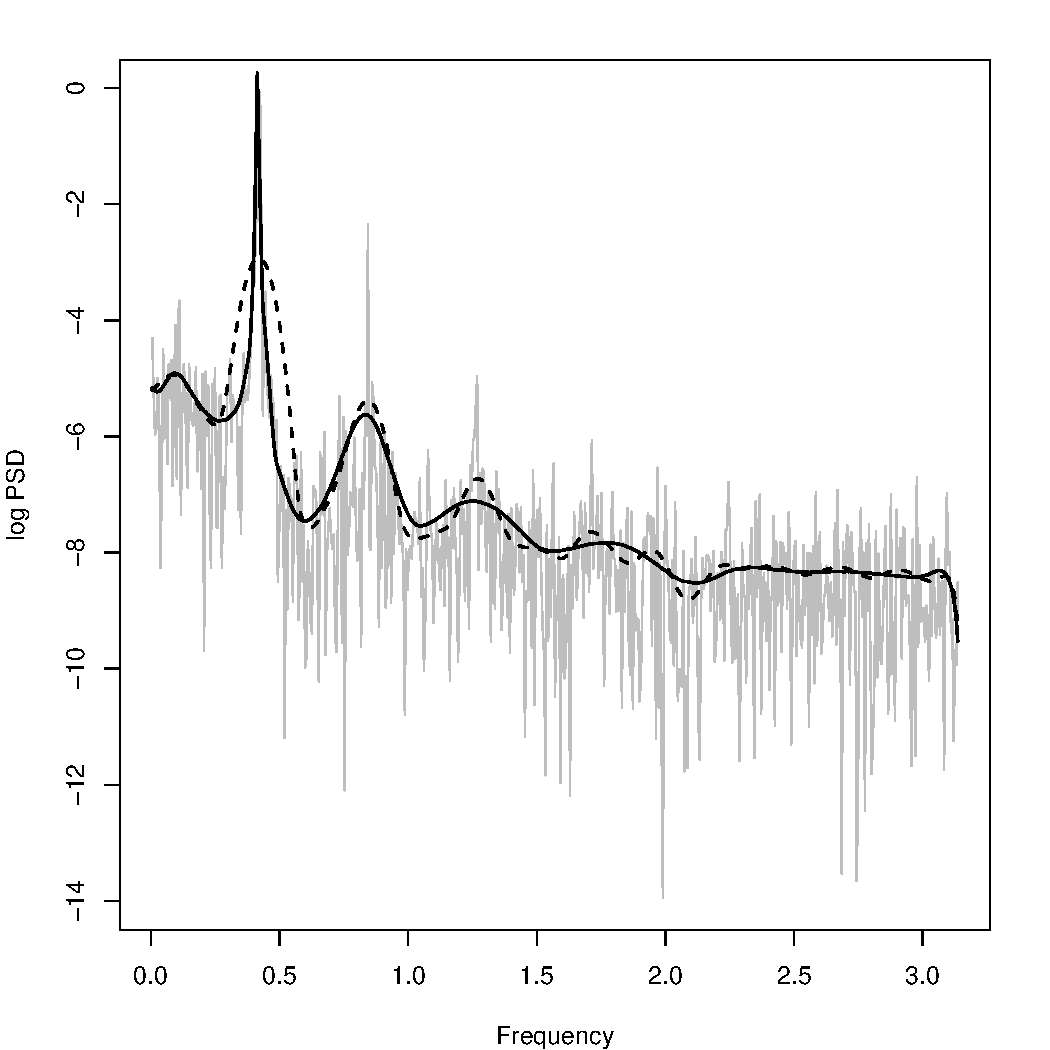
\includegraphics[scale=0.5,clip=true,angle=0]{carinae.pdf}
	\caption{Log-spectral density estimate for the variable star S. Carinae data via the P-spline prior algorithm. The continuous gray line represents the periodogram whereas the continuous and dashed black lines stand for the posterior median log-PSD obtained using the periodogram knot location scheme and equally spaced knots, respectively.}
	\label{fig:carinae}
\end{figure}

The periodogram shows several peaks, being the main one located at around 0.42.  When the knots are equally spaced, the algorithm is unable to capture properly this characteristic, unlike our knot location proposal.  This is because our approach allocates more knots in those areas which contain significant peaks detected via the periodogram.  The rest of peaks, which are smaller in comparison to the main one, are slightly better captured by the equally spaced knot approach, since the other scheme spend most of the effort in the main peak, but which can be corrected by increasing the number of knots.  Allowing the knots to vary according to the periodogram, the PSD estimate is more similar to the one obtained via the NPC approach \citep{Kirch:2018}.

\section{Discussion}

As shown by \cite{Edwards2018}, the B-spline prior outperforms the Bernstein polynomial prior in terms of IAE and uniform coverage probabilities for complicated PSDs.  This is explained by the local support of the B-splines and its better approximation properties \citep{Edwards2018}.  However, its performance involves a much higher computational cost.  These characteristics have motivated our approach.  

The P-spline prior can be considered a particular case of the B-spline prior.  The latter works with a variable number and location of knots, which are driven by the data.  The P-spline prior assumes a fixed number of knots, with fixed locations.  These simplifications reduce the computational effort significantly, without sacrificing accuracy as shown in the application section.  To deal with abrupt peaks in the PSD, we propose to locate the knots according to the peaks detected via the periodogram.  This approach does not affect the computational time and improve the estimates dramatically.

In our simulation study, we showed that, in general, the P-spline prior outperforms the B-spline prior in all our assessments, that is in terms of IAE, coverage probabilities, and run-times.  From this example, it seems that a second order penalty P-spline works reasonably well.

We also assessed our proposal in the classic sunspot dataset, in which the B-spline prior algorithm is able to estimate correctly the solar cycle that occurs every 11.07 years.  The P-spline prior yields almost identical results, but in a significant less computational time.  

Finally, we assess the P-spline prior algorithm under two different knot location schemes: equally spaced and distributed according to the periodogram.  For this, we estimated the PSD for the S. Carinae data, which function contains several abrupt peaks.  The equal spaced scheme fails in capturing the peaks of the function.  On the other hand, our proposal improved significantly the results without affecting the computational time.

The number of B-spline densities was selected according to the criterion proposed by \cite{Ruppert2002}.  It seems to work well, at least for the kind of PSDs treated in this work.  However, more complex functions could require larger number of B-spline densities.  This can be evaluated studying the peaks of the periodogram.  Our knot location proposal is very useful in these situations.

In conclusion, the P-spline prior represents a more viable alternative to the B-spline prior for spectral density estimation.  As shown in this work, it can handle quite well complex PSDs in a reasonable time-run.\\

\begin{acknowledgements}
  We thank the New Zealand eScience Infrastructure (NeSI) for their high performance computing facilities, and the Centre for eResearch at the University of Auckland for their technical support. PM's and RM's work is supported by Grant 3714568 from the University of Auckland Faculty Research Development Fund and the DFG Grant KI 1443/3-1.  All analysis was conducted in \textsf{R}, an open-source statistical software available on \textsf{CRAN} (cran.r-project.org).
\end{acknowledgements}

%\pagebreak

%%%%%%%%%%

\bibliographystyle{apsrev4-1}

\bibliography{pSplinesReferences}

\end{document}

%\begin{thebibliography}{10}

%\end{thebibliography}
%%%%%%%%%%

\end{document}
